% !TEX encoding = UTF-8
% !TEX TS-program = pdflatex
% !TEX root = ../tesi.tex

\chapter{Analisi del contesto aziendale}
\label{cap:contesto-aziendale}

% !TEX encoding = UTF-8
% !TEX TS-program = pdflatex
% !TEX root = ../../tesi.tex

\section{L'azienda Sync Lab}
Sync Lab nasce come \textit{software house} nel 2002, per poi crescere rapidamente nel mercato del \gls{ICT}. In seguito ad una maturazione delle competenze tecnologiche, metodologiche ed applicative nel dominio del \textit{software}, si è tramutata in \gls{System Integrator} conquistando significative fette di mercato nei settori: \textit{mobile}, videosorveglianza e sicurezza delle infrastrutture informatiche aziendali. Attualmente possiede più di 150 clienti diretti e finali, 200 dipendenti e 5 sedi distribuite in tutta Italia. 

\begin{figure}[!h]
  \centering
  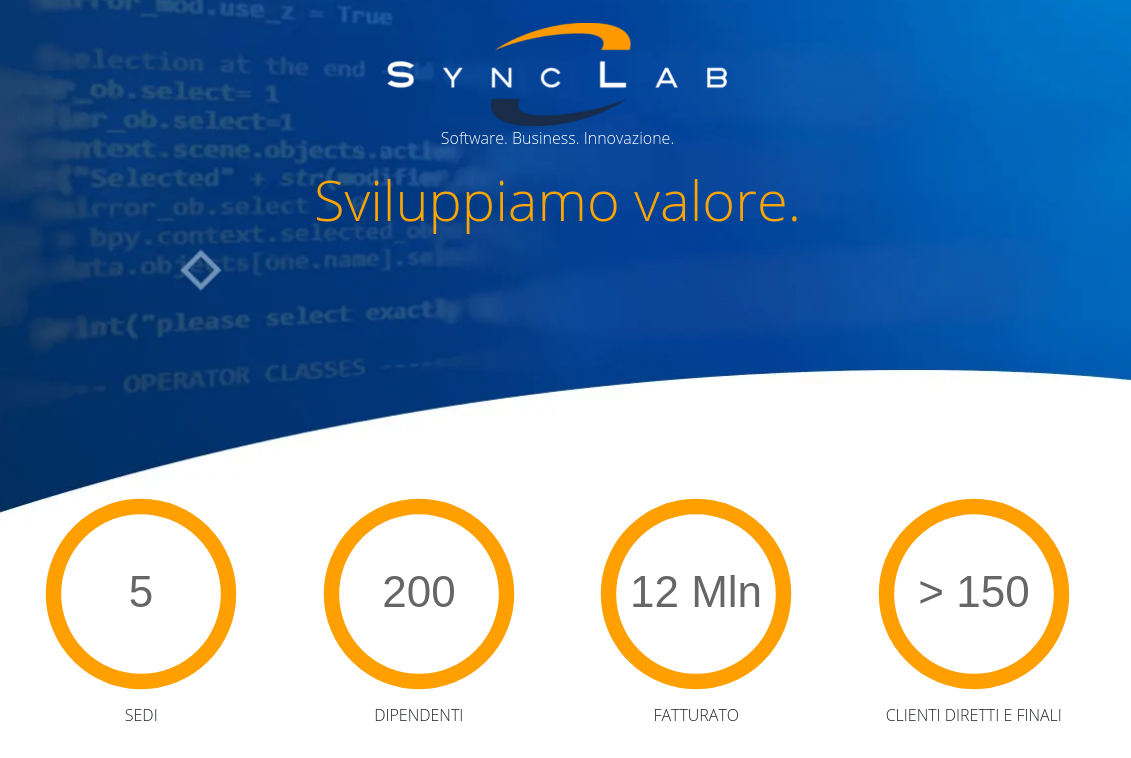
\includegraphics[width=\textwidth]{capitolo1/motto-synclab.png}
  \caption{Motto di Sync Lab e le sue statistiche}
  \textbf{Fonte}: \href{https://www.synclab.it}{https://www.synclab.it}
\end{figure}

Sync Lab consegue l'obiettivo principale di supportare il cliente nella realizzazione, messa in opera e controllo di soluzioni \textit{IT}, sia dal punto di vista tecnologico, sia nel governo del cambiamento organizzativo. Nel corso degli anni ha aumentato la propria qualità organizzativa e produttiva, riuscendo ad acquisire le seguenti 4 certificazioni: ISO 9001, ISO 14001, ISO 27001 e ISO 45001.





% !TEX encoding = UTF-8
% !TEX TS-program = pdflatex
% !TEX root = ../../tesi.tex

\section{Prodotti}
Per quanto concerne i prodotti, ho discusso con il mio \textit{tutor} aziendale, Fabio Pallaro, il quale mi ha specificato che tutti i prodotti sono stati sviluppati per aiutare le aziende ad affrontare i cambiamenti tecnologici e di mercato, rimanendo sempre competitive nell'attuale contesto di trasformazione digitale. I settori informatici dove opera principalmente l'azienda sono: il \textit{business consultancy}, il \textit{IT consultancy} e il \textit{project financing}.

\begin{figure}[!h]
  \centering
  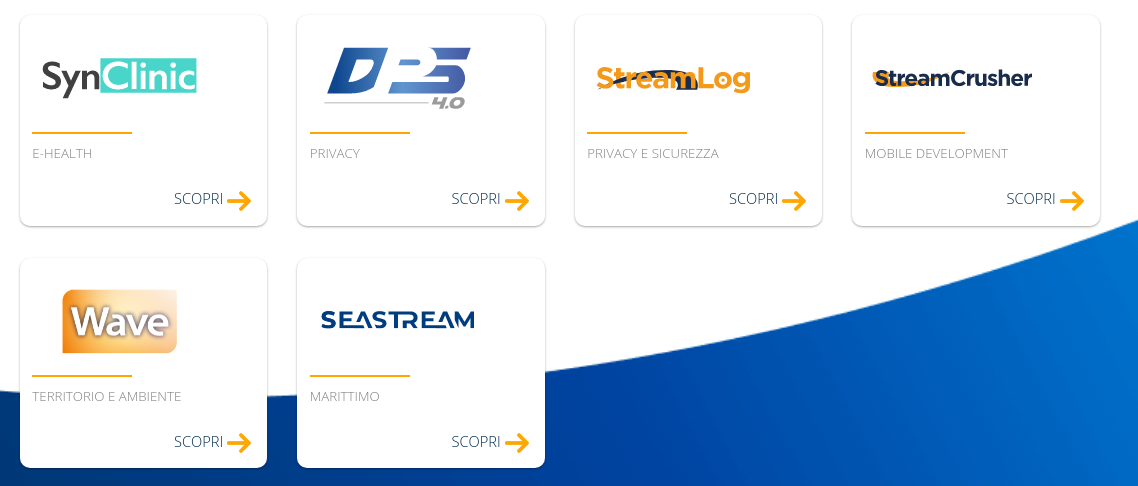
\includegraphics[width=\textwidth]{capitolo1/prodotti-synclab.png}
  \caption{I prodotti di Sync Lab}
  \textbf{Fonte}: \href{https://www.synclab.it/prodotti.php}{https://www.synclab.it/prodotti.php}
\end{figure}

\noindent In questo ambito, Sync Lab, ha sviluppato numerosi prodotti:
\begin{itemize}
  \item \textbf{SynClinic}: \textit{software} che facilita la gestione di una struttura sanitaria. Utilizzabile in \textit{cloud} e \gls{on premises}, gestisce, organizza e monitora tutte le fasi del percorso di cura del paziente, integrandosi perfettamente con i servizi regionali: fascicolo sanitario elettronico, ricetta dematerializzata e CUP regionale;
  
  \item \textbf{DPS 4.0}: consiste in una soluzione web per la gestione del GDPR, con una piattaforma guidata per aggiornare e modificare automaticamente i documenti di privacy in modo conforme agli standard di riferimento europei;
  
  \item \textbf{StreamLog}: rappresenta un sistema finalizzato al soddisfacimento dei requisiti fissati al garante, ovvero effettua il controllo degli accessi ai sistemi in modo semplice e veloce. La piattaforma è basata su \textit{framework open source} allo stato dell'arte e, in particolare, su un'innovativa tecnologia di \textit{streaming}, frutto del laboratorio di ricerca e sviluppo Sync Lab;
  
  \item \textbf{StreamCrusher}: soluzione \textit{software} che è in grado di raccogliere, indicizzare, ed interpretare la grande mole di dati che giornalmente genera qualsiasi azienda. In seguito, produrrà un resoconto con tutte le informazioni utili al centro informatico, per identificare criticità o eventuali opportunità di \textit{business};
  
  \item \textbf{Wave}: nato dal laboratorio di ricerca e sviluppo, è un \textit{plugin} della piattaforma \textit{Milestone System A/S} che permette di avere una visione geografica della distribuzione delle telecamere installate nel territorio e di capire la copertura garantita da un'installazione reale;
  
  \item \textbf{SeaStream}: piattaforma che migliora l'efficienza, la sicurezza e il processo di innovazione del settore marittimo, mettendo a disposizione strumenti per il monitoraggio e tracciamento delle navi e per la gestione portuale.  
\end{itemize}

% !TEX encoding = UTF-8
% !TEX TS-program = pdflatex
% !TEX root = ../../tesi.tex

\section{Tipologia di clientela}
La clientela che si affida a Sync Lab è molto vasta, comprendendo al suo interno aziende pubbliche e private, piccole e grandi imprese. Tutte le aziende elencate in precedenza si mettono in contatto con Sync Lab per migliorare i propri processi interni, andando così ad incrementare la propria efficienza sotto l'aspetto lavorativo. Riuscendo a soddisfare qualsiasi richiesta, Sync Lab può vantare clienti come: la regione Lazio, Trenitalia, il ministero dell'economia e delle finanze, Rai, Unicredit, Vodafone e Intesa San Paolo. Per ogni settore, l'azienda è in continua ricerca di nuove opportunità e soluzioni cercando di allargare sempre più il proprio campo applicativo per portare verso di sè una clientela più varia.


% !TEX encoding = UTF-8
% !TEX TS-program = pdflatex
% !TEX root = ../../tesi.tex

\section{Processi aziendali}
Sync Lab conta di raggiungere i propri obiettivi aziendali attraverso i processi spiegati di seguito.

\subsection{Consulenza}

\begin{figure}[!h]
  \centering
  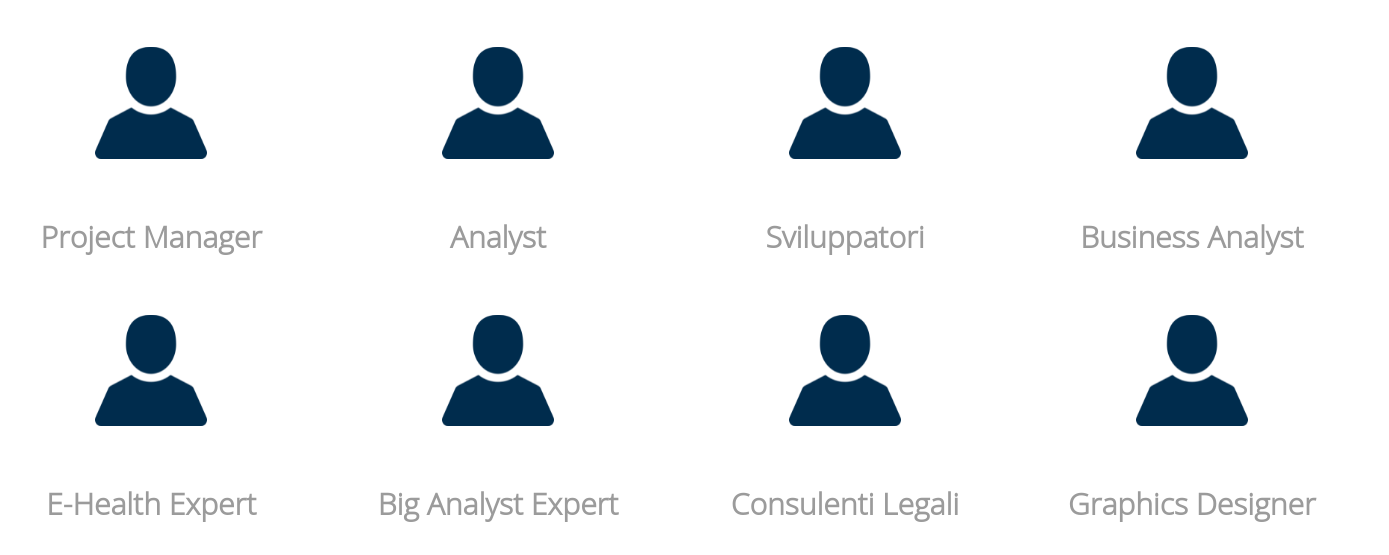
\includegraphics[width=\textwidth]{capitolo1/profili-professionali.png}
  \caption{I profili professionali messi a disposizione da Sync Lab}
  \textbf{Fonte}: \href{https://www.synclab.it/servizi-professionali.php}{https://www.synclab.it/servizi-professionali.php}
\end{figure}

In quanto \textit{partner} di grandi imprese italiane, come spiegato nella sezione precedente, uno degli obiettivi principali di Sync Lab è quello di fornire una consulenza ai suoi clienti che porti un'evoluzione in termini di competitività, sviluppo e innovazione tecnologica. Inoltre, mette a disposizione un team di grande esperienza che interviene nella progettazione e realizzazione delle strategie necessari alla realizzazione di grandi progetti.

\subsection{Fornitura}
La procedura di fornitura viene avviata ogni qual volta che un cliente incarica Sync Lab per la realizzazione di un prodotto. Parallelamente, mette in atto le seguenti attività con lo scopo di migliorare questo processo:
\begin{itemize}
  \item \textbf{Miglioramento delle performance}: verifica e correzione, se necessario, delle procedure aziendali utilizzando le giuste metodologie (\textit{best practices});
  \item \textbf{Ottimizzazione della qualità}: utilizzo di \textit{design patterns} adatti al contesto aziendale;
  \item \textbf{Sviluppo delle quote di mercato}: analisi e miglioramento degli standard di qualità presso l'azienda.
\end{itemize} 

\subsection{Sviluppo}
Sync Lab fa ampio uso del modello di sviluppo Agile, più in particolare della metodologia Scrum, per permettere agli \textit{stakeholders} di seguire l'evoluzione dello sviluppo del prodotto richiesto, raccogliendo tutti i \textit{feedback} che possono essere determinanti per la loro soddisfazione. 

\paragraph{La metodologia Scrum}
Scrum è la metodologia Agile più diffusa tra i team di sviluppo. In questa metodologia gli \textit{stakeholders} hanno un ruolo fondamentale e la loro soddisfazione è determinante per la buona riuscita del progetto. Per rispondere al meglio a questa esigenza, si basa su tre pilastri fondamentali:
\begin{enumerate}
  \item \textbf{Trasparenza}: tutti coloro che partecipano ad un progetto sanno qual è lo scopo (trasparenza verticale) e sanno che cosa fanno gli altri (trasparenza orizzontale). In più, anche lo stato del progetto, con le relative statistiche, è visibile a tutti a prescindere dal livello organizzativo;
  \item \textbf{Ispezione}: ogni iterazione ed incremento vengono verificati in base alle metriche di misurazione decise, in modo tale da modificare le iterazioni successive e rendere così estremamente adattabile l'andamento del processo;
  \item \textbf{Adattamento}: è la conseguenza dell'ispezione e significa che al posto di seguire un piano preordinato, il team di sviluppo pianifica in base ai risultati dell'ispezione per apportare il maggior valore al cliente finale.
\end{enumerate}

\clearpage

\begin{figure}[h!]
  \centering
  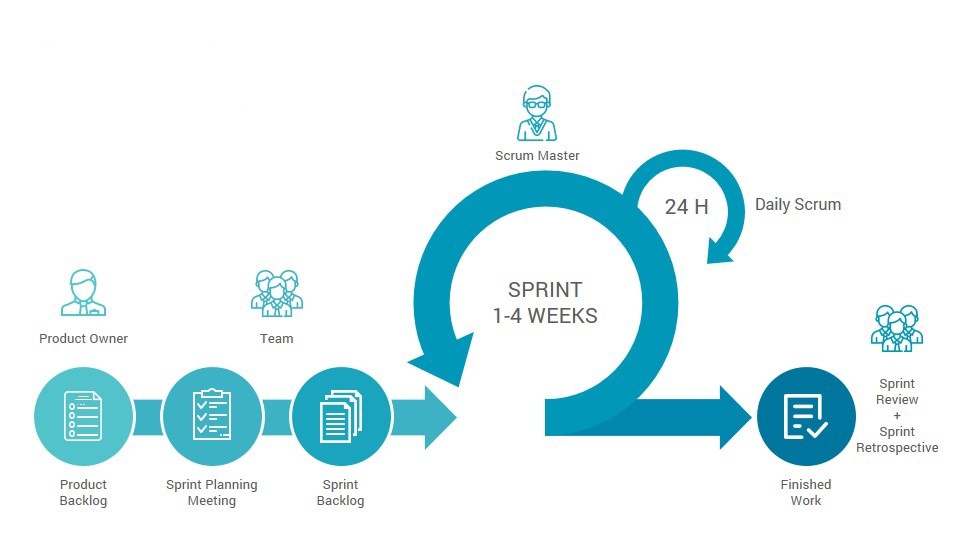
\includegraphics[width=0.8\textwidth]{capitolo1/scrum.jpeg}
  \caption{La metodologia Scrum}
  \textbf{Fonte}: \href{https://medium.com/swlh/agile-primer-for-non-technical-teams-1deb06968281}{https://medium.com/swlh/agile-primer-for-non-technical-teams}
\end{figure}

Durante il periodo di stage ho potuto osservare come vengono organizzati e gestiti i vari \textit{sprint} in Sync Lab. Ad ogni \textit{sprint} corrisponde l'introduzione di una nuova funzionalità che viene opportunamente verificata e comprovata dalla soddisfazione del cliente. L'esecuzione di uno \textit{sprint} prevederà i seguenti passi:
\begin{enumerate}
  \item si definisce un \textbf{\textit{product backlog}}, dove verranno riportate le attività da fare in una \textit{scrum board}, relative al progetto;
  \item si realizza uno \textbf{\textit{sprint planning}}, un sottoinsieme di obiettivi da raggiungere durante un singolo \textit{sprint} sulla base del \textit{product backlog};
  \item si esegue lo \textbf{\textit{sprint}} in un lasso di tempo limitato di massimo 4 settimane;
  \item si revisiona lo \textbf{\textit{sprint goal}} in cui si valuta l'incremento effettivo al termine dello \textit{sprint}.
\end{enumerate}

% \clearpage

\begin{figure}[h!]
  \centering
  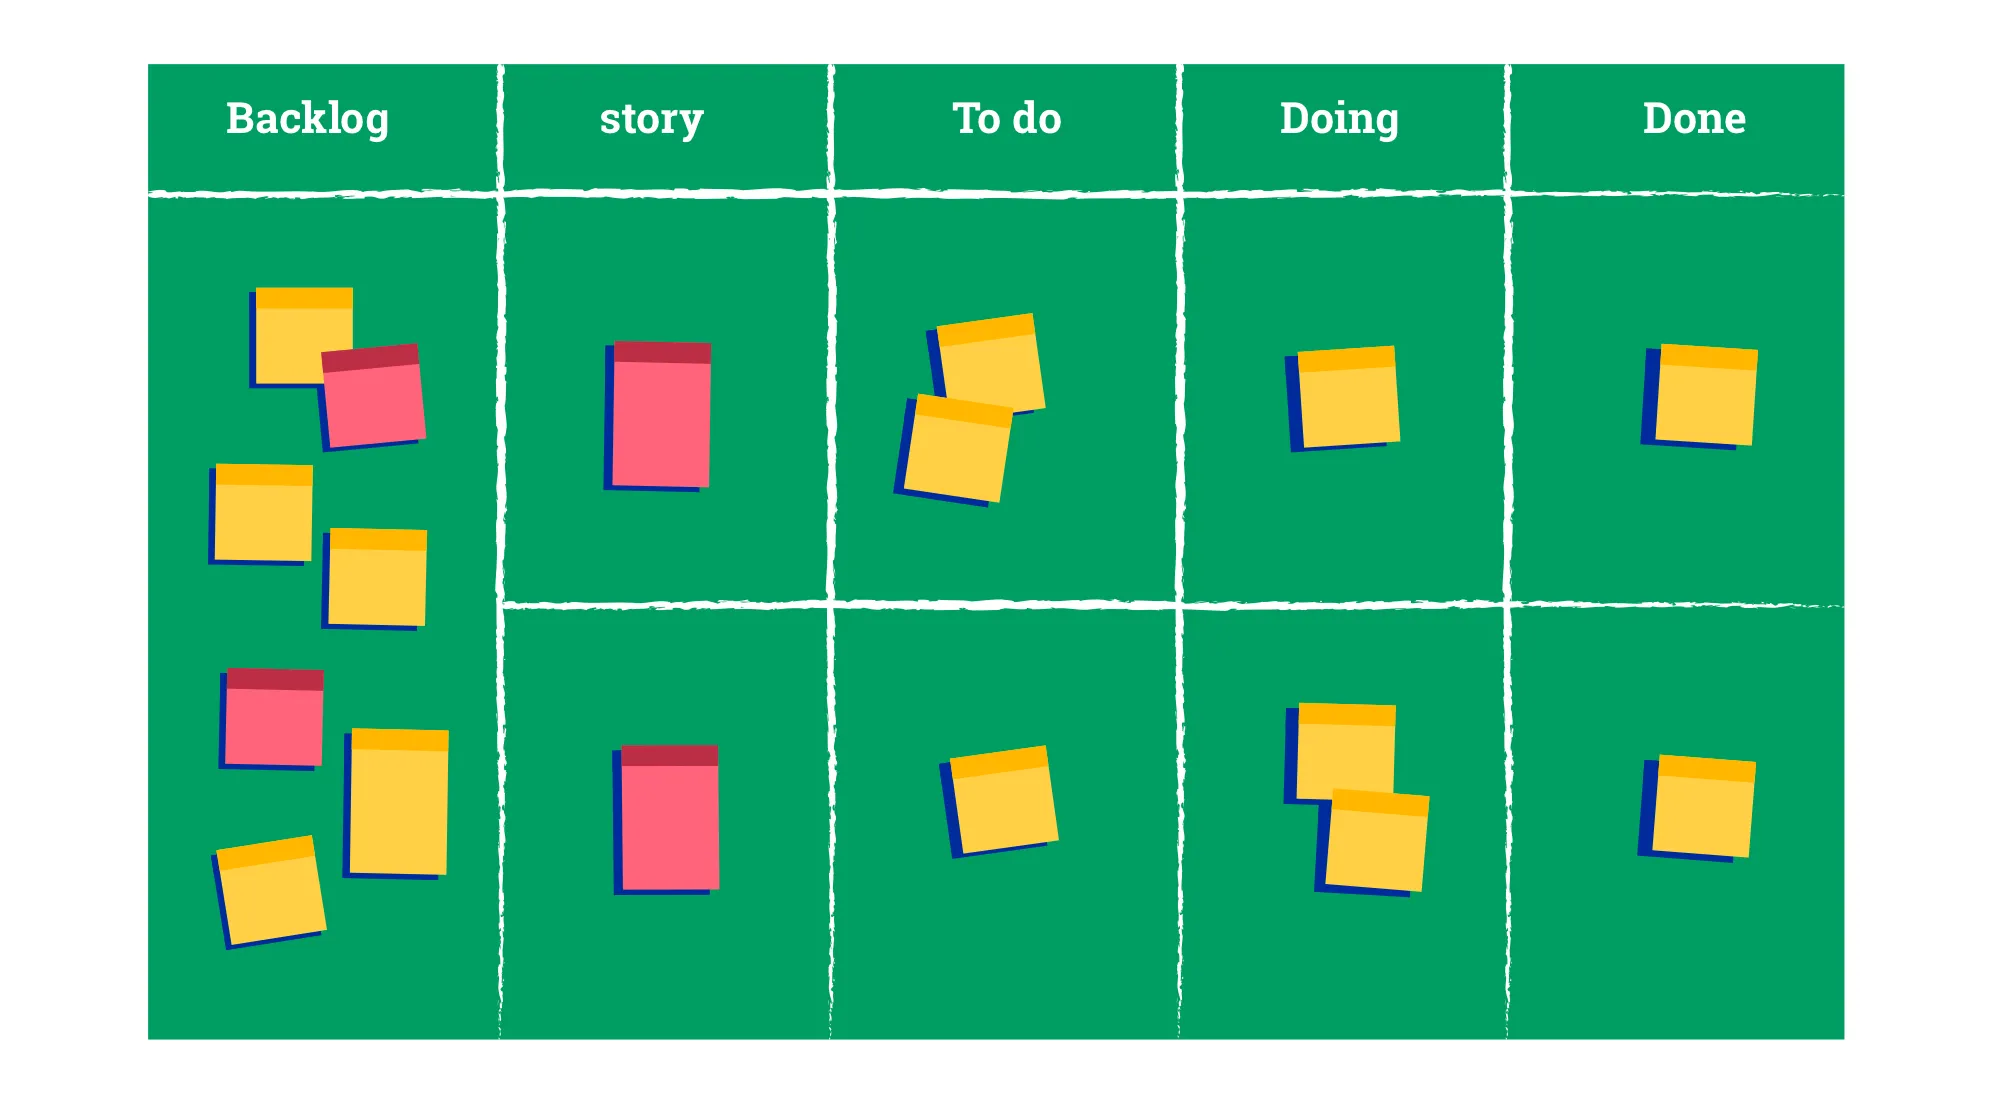
\includegraphics[width=0.8\columnwidth]{capitolo1/scrumb-board.png}
  \caption{Esempio di organizzazione delle attività nella Scrum Board}
  \textbf{Fonte}: \href{https://www.zoho.com/sprints/what-is-a-scrum-board.html}{https://www.zoho.com/sprints/what-is-a-scrum-board.html}
\end{figure}

Un altro evento fondamentale che fa parte di Scrum, al quale ho avuto modo di partecipare, è lo \textbf{\textit{sprint review}}. Quest'ultimo consiste in una riunione di fine sprint in cui si ispezionano i risultati dell'incremento insieme agli \textit{stakeholders}, decidendo eventuali cambiamenti da apportare al \textit{product backlog}. \\

\subsection{Manutenzione}
In seguito al rilascio di un \textit{software}, l'azienda si impegna a seguire la sua naturale evoluzione nel tempo, adattandolo sempre a nuove esigenze, e a risolvere eventuali errori. Per questo Sync Lab offre servizi di manutenzione che possono essere di tre tipi:
\begin{itemize}
  \item \textbf{Manutenzione correttiva}: permette di correggere eventuali difetti del prodotto;
  \item \textbf{Manutenzione adattiva}: permette di adattare il \textit{software} a cambiamenti dell'ambiente operativo;
  \item \textbf{Manutenzione evolutiva}: permette di estendere le funzionalità del prodotto esistente.
\end{itemize}

% !TEX encoding = UTF-8
% !TEX TS-program = pdflatex
% !TEX root = ../../tesi.tex

\section{Tecnologie utilizzate}
\label{sec:tecnologie-utilizzate}

Da quel che ho potuto constatare durante l'attività di stage, per la realizzazione dei prodotti sopra elencati Sync Lab sfrutta un'ampia gamma di tecnologie per fornire prodotti stabili e sicuri. Le tecnologie utilizzate sono molte e variano in base alla necessità del prodotto, ma quelle più utilizzate possono essere raggruppate in due grandi categorie: \textit{front-end} e \textit{back-end}. \\

Per quanto riguarda le tecnologie di supporto, c'è stato un aumento di utilizzo dei sistemi di comunicazione digitali a causa della pandemia, anche se venivano già utilizzati precedentemente per comunicare con le diverse sedi. La pandemia ha spinto Sync Lab ad un utilizzo sempre maggiore di Discord, Google Meet, Trello e Notion.

\begin{itemize}
  \item \textbf{Google Meet}: \textit{software} utilizzato per le videoconferenze che permette di comunicare con più colleghi e organizzare riunioni virtuali con un grande numero di partecipanti;
  \item \textbf{Discord}: piattaforma di comunicazione digitale gratuita, la quale permette di fruire di chat in tempo reale, gestendo più canali vocali e testuali divisi per argomento. Tra le varie funzioni disponibili, permette di dividere i membri in gruppi in base al progetto che devono portare a termine. È presente anche una sezione per le videoconferenze, ma è meno avanzata rispetto a Google Meet e per questo non lo si preferisce;
  \item \textbf{Trello}: piattaforma per la gestione di progetti seguendo la metodologia Scrum. Trello mette a disposizione una \textit{Scrum Board} dove è possibile dividere le attività in base al loro stato di avanzamento. Le colonne sono modificabili, come qualsiasi componente in Trello, ma quelle predefinite sono le seguenti:
  \begin{itemize}
    \item \textbf{\textit{Backlog}}: contiene il \textit{product backlog};
    \item \textbf{Da fare}: definisce le attività da svolgere durante lo \textit{sprint};
    \item \textbf{In corso}: presenta tutte le attività in esecuzione;
    \item \textbf{In verifica}: consiste in tutte le attività in attesa di verifica;
    \item \textbf{Terminati}: include le attività legate ad uno \textit{sprint} che sono state verificate. 
  \end{itemize}
  \item \textbf{Notion}: piattaforma utilizzata per la prenotazione del posto in sede, così da facilitare la gestione ed il controllo delle persone, in modo tale da rispettare il numero massimo consentito dalla legge.
\end{itemize}

\subsection{Front-end}
Le tecnologie per lo sviluppo di interfacce grafiche utilizzate da Sync Lab sono le seguenti:

\paragraph{Linguaggi di programmazione} 
I linguaggi di programmazione più utilizzati sono:
\begin{itemize}
  \item \textbf{HTML5}: anche se non è prettamente un linguaggio di programmazione, ma bensì un linguaggio di \textit{markup}, viene utilizzato dall'azienda Sync Lab per la strutturazione delle sue pagine web. Ha lo scopo di definire la struttura grafica, ovvero il \textit{layout}, tramite l'utilizzo di \textit{tag} diversi;
  
  \item \textbf{CSS3}: è un linguaggio che viene utilizzato per definire la formattazione di documenti HTML. Sync Lab lo ha adottato per mantenere separati i contenuti della pagina, dalla loro presentazione;

  \item \textbf{Javascript}: impiegato nella realizzazione di applicativi web interattivi, è diventato in questi ultimi anni il linguaggio di programmazione più utilizzato al mondo. Questo è stato causato dalla grande diffusione che ha avuto il web, dalla sua semplicità d'uso e, in particolare, dalla non presenza di concorrenti in questo settore. Javascript si basa sui paradigmi di programmazione ad oggetti e a eventi, ma ha il grande difetto di non avere la tipizzazione statica delle variabili, ovvero non viene specificato il tipo delle variabili durante la scrittura del codice. A causa di questa mancanza molto grave che provoca svariati problemi quando in seguito il codice verrà eseguito, molti sviluppatori si stanno spostando verso \textbf{Typescript}, ovvero un \textit{superset} di Javascript, il quale aggiunge la tipizzazione statica del codice, una sintassi più aggiornata per la scrittura delle classi e delle interfacce e molti altri costrutti che facilitano la scrittura del codice. Per \textit{superset} si intende che il codice scritto in Typescript viene tradotto in codice Javascript attraverso un processo di transpilazione. Questo permette a codice Typescript di essere eseguito su qualsiasi browser, o generalizzando, qualsiasi macchina virtuale che esegue codice Javascript;
  
  \item \textbf{Kotlin}: un linguaggio multi-paradigma che è sempre più diffuso per lo sviluppo di applicazioni android, il quale sta andando a sostituire Java. Kotlin è molto più semplice e veloce rispetto a Java, infatti qualsiasi pezzo di codice scritto in Kotlin è notevolmente più corto. Questo permette, auspicabilmente, di introdurre meno \textit{bug} nel codice. Inoltre, Kotlin risolve il problema del \textit{NullPointerException} che in Java crea numerosi inconvenienti. Per fare ciò, in Kotlin sono stati introdotti due tipi di variabili: i \textit{nullable types} e i \textit{non-nullable types}. In poche parole, tutte le variabili quando vengono dichiarate sono di tipo \textit{non-nullable} e non possono avere valore \textit{null}. Per far si che possa assumere valore \textit{null} bisogna dichiarare la variabile con una sintassi apposita. Per questi motivi e molti altri, Kotlin è stato adottato dall'azienda per lo sviluppo di applicazioni Android.
\end{itemize}

\paragraph{Framework} L'ambito web è quello dove avviene un impiego maggiore di \textit{framework}. I più utilizzati attualmente sono:
\begin{itemize}
  \item \textbf{Angular}: è uno dei \textit{framework} open-source più popolari e utilizzati al mondo per lo sviluppo di \gls{Single Page Application}. Permette di creare applicazioni web di livello \textit{enterprise} grazie alla sua architettura \textit{MVC} (\textit{Model View Controller}) utilizzando come linguaggio principale Typescript. Angular è stato il primo \textit{framework} a rendere disponibile anche per lo sviluppo web, vari \textit{design pattern}, tra i quali il più importante è il \textit{dependency injection}. In Angular tutto viene trattato come un componente e questo permette la riduzione della duplicazione del codice e aumenta di molto la riusabilità;
  
  \item \textbf{React.js}: si distingue da Angular per la maggiore facilità di apprendimento e velocità a livello di \textit{performance}, la quale lo rende perfetto per la realizzazione di siti semplici. Anche React si basa sul concetto di componente, ma non utilizza alcuna architettura MVC. Infatti React utilizza l'architettura \textit{Flux/Redux}, creata appositamente per quest'ultimo. La velocità di React è data dall'utilizzo di un \textit{Virtual DOM}, un \textit{DOM} locale al sito al cui vengono applicate le modifiche che bisogna compiere alla vista, per identificare le modifiche finali ed applicarle al \textit{DOM} reale, così da evitare tutti i cambiamenti intermedi;
  
  \item \textbf{Vue.js}: molto simile a React.js, Vue.js introduce il concetto di \gls{Single File Components}, semplificando maggiormente la scrittura di applicazioni web. Sempre basato sul concetto di componenti e riusabilità, è utilizzabile anche con il linguaggio Typescript e si basa sul \textit{Virtual DOM} come React.js. Vue.js è un \textit{framework} che sta sempre di più prendendo piede all'interno dell'azienda, anche se di fatto non è ancora stato adottato ufficialmente.
\end{itemize}

\subsection{Back-end}
Per quanto riguarda le tecnologie per lo sviluppo lato \textit{back-end}, si possono identificare le seguenti:

\paragraph{Linguaggi di programmazione}
I linguaggi più utilizzati per lo sviluppo lato \textit{back-end} sono entrambi basati sulla \textit{Java Virtual Machine}:
\begin{itemize}
  \item \textbf{Java}: essendo il linguaggio per lo sviluppo di \textit{back-end} più utilizzato al mondo, ha il vantaggio di avere a disposizione una \textit{community} molto vasta e un elevato numero di \textit{framework} stabili ed impiegati per moltissimi applicativi. Oltre ad essere un linguaggio di programmazione multi-paradigma orientato agli oggetti e avere la tipizzazione statica, ha il vantaggio di essere stato progettato con l'obiettivo di essere il più possibile indipendente dalla piattaforma \textit{hardware} di esecuzione. Infatti il codice Java non viene tradotto in codice macchina da un compilatore, ma verrà compilato in \textit{bytecode} per essere eseguito dalla macchina virtuale \textit{Java Virtual Machine}. Viene impiegato principalmente per la scrittura di servizi con architettura \textit{REST}, ovvero con una struttura ben definita dove ogni servizio non ha sessioni, ha degli \textit{URL} a cui fanno riferimento delle \textit{API} e si utilizzano dei metodi specifici per il recupero di informazioni, per la modifica e altri scopi;
  
  \item \textbf{Scala}: è un linguaggio che si basa sui paradigmi di programmazione ad oggetti e funzionale, con la caratteristica di avere una tipizzazione forte. Viene impiegato dall'azienda per lo sviluppo di applicazioni concorrenti, distribuite, resilienti e guidate dai messaggi, oppure per la scrittura di librerie che in seguito verranno integrate con Java.
\end{itemize}

\paragraph{Framework} Il \textit{framework} più utilizzato per lo sviluppo in questo ambito è sicuramente \textbf{Spring}. Quest'ultimo permette di realizzare applicativi lato \textit{server} utilizzando il linguaggio Java e sfruttando vari \textit{design pattern}. A Spring vengono associati altri progetti tali Spring Boot, Spring Data, Spring Batch, Spring MVC. La scelta dell'architettura è totalmente libera e Spring si presta perfettamente a qualunque tipologia si voglia scegliere. 
Sync Lab lo impiega per lo sviluppo di architetture a micro-servizi, con l'utilizzo del \textit{MVC pattern}.

% !TEX encoding = UTF-8
% !TEX TS-program = pdflatex
% !TEX root = ../../tesi.tex

\section{Propensione all'innovazione}
Sync Lab è un'azienda in costante aggiornamento che guarda all'innovazione con grande interesse, per garantire soluzioni software sempre rivoluzionarie. Simbolo di questo sforzo da parte dell'azienda è anche la grande quantità di collaborazioni con le principali università d'Italia (Università degli Studi di Padova, Politecnico di Milano, Università degli Studi Federico II, ecc.) e vari enti europei. \\

\begin{figure}[!h]
  \centering
  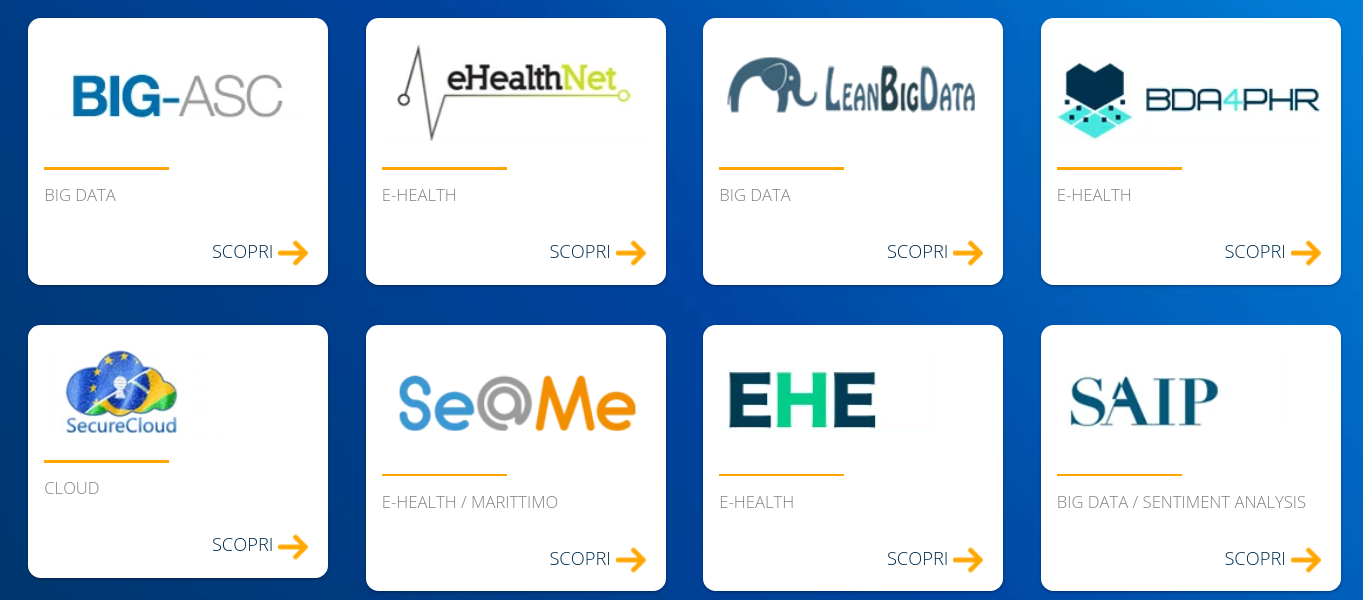
\includegraphics[width=\textwidth]{capitolo1/prodotti-ricerca-sviluppo.png}
  \caption{Alcuni progetti di ricerca e sviluppo di Sync Lab}
  \textbf{Fonte}: \href{https://www.synclab.it/ricerca-e-sviluppo.php}{https://www.synclab.it/ricerca-e-sviluppo.php}
\end{figure}

Per adempiere al meglio al difficile compito di restare sempre aggiornati sulle ultime tecnologie, Sync Lab è divisa in tre dipartimenti:
\begin{itemize}
  \item \textbf{\textit{Research and Development (R\&D)}}: dove l'azienda promuove nuovi prodotti eseguendo ricerca e sviluppo in più settori, alimentando così il profilo aziendale e le proprie competenze nel mercato;
  \item \textbf{\textit{Lab}}: in cui l'azienda mette in atto i risultati derivanti dal dipartimento \textit{R\&D}, promuovendo soluzioni che migliorino ed estendano l'innovazione tecnologica;
  \item \textbf{\textit{Start-up}}: dove l'azienda collabora e promuove le \textit{start-up} con maggiore successo in termini di innovazione, sia in Italia che all'estero.
\end{itemize}  

L'azienda, inoltre, sta approfondendo sempre di più gli ambiti di \textit{Cybersecurity}, \textit{E-Health}, \textit{Blockchain} e \textit{Big Data}, formando degli appositi progetti di ricerca nelle diverse sedi per sperimentare e imparare nuove tecnologie. \\

Un evento che ho trovato interessante e mi è piaciuto molto durante il mio tirocinio, è stato il "Paola presenta". 
Questa ricorrenza, che in genere è settimanale, consiste in un'ora di presentazione su un argomento proposto da un dipendente. L'argomento della presentazione può riguardare qualcosa sulla quale sta lavorando, oppure semplicemente si è interessato. 
Ogni dipendente è libero di partecipare e, su richiesta, può presentare lui stesso un argomento a piacere. Questo evento l'ho trovato molto interessante e dimostra quanto i colleghi di Sync Lab vogliano sempre stare aggiornati ed informati su tutto quello che interessa il mondo informatico. 
Personalmente ho partecipato a tre di queste presentazioni: una dove hanno introdotto la tecnologia \textit{Blockchain}, tenuta dal mio \textit{tutor} aziendale Fabio Pallaro, un'altra dove hanno spiegato come funzionano gli strumenti che compongono la \textit{Elastick Stack} e l'ultima dove hanno parlato dell'analisi statica del codice con la piattaforma \textit{SonarQube}. \\

Questa propensione all'innovazione l'ho avvertita anche nel mio progetto di stage, dove non ho trattato tecnologie usuali, ma ho dovuto studiare e approfondire tecnologie che attualmente non sono così diffuse in ambito \textit{enterprise}, ma sicuramente rappresentano un'importante \textit{milestone} nella storia dell'informatica.
